\begin{frame}{Introduction}{State-of-affairs and motivation}
	\begin{itemize}
		\item Global energy demand is still rising
		\item Wind energy is a part of solution to lower CO2 emissions
		\item LCOE higher in offshore wind turbines but there are advantages
		\item Shallow-water depth sites (<50 m) will eventually exhaust
		\item Floating turbines are in prototype stage but maturing
		\item In recent news: "\textit{Portugal to auction 3-4 GW of floating offshore wind farms in summer}" (\href{https://www.reuters.com/business/energy/portugal-auction-3-4-gw-floating-offshore-wind-farms-summer-2022-03-16/}{Article link})
	\end{itemize}\bigskip
\end{frame}

%%%%%%%%%%%%%%%%

\begin{frame}{Introduction}{Floating offshore wind turbines (FOWTs)}
	\begin{columns}
		\begin{column}{.49\textwidth}
			\begin{itemize}
				\item Experiences higher strain mainly due to extra degrees of freedom
				\item Fore-aft motion: Surge \& pitch
				\item Load reduction $ \rightarrow $ LCOE reduction $ \rightarrow $ greater economical feasibility
			\end{itemize}
		\end{column}
		
		\begin{column}{.49\textwidth}
			The 6 additional degrees of freedom of a FOWT:
			\begin{figure}[ht]
				\centering
				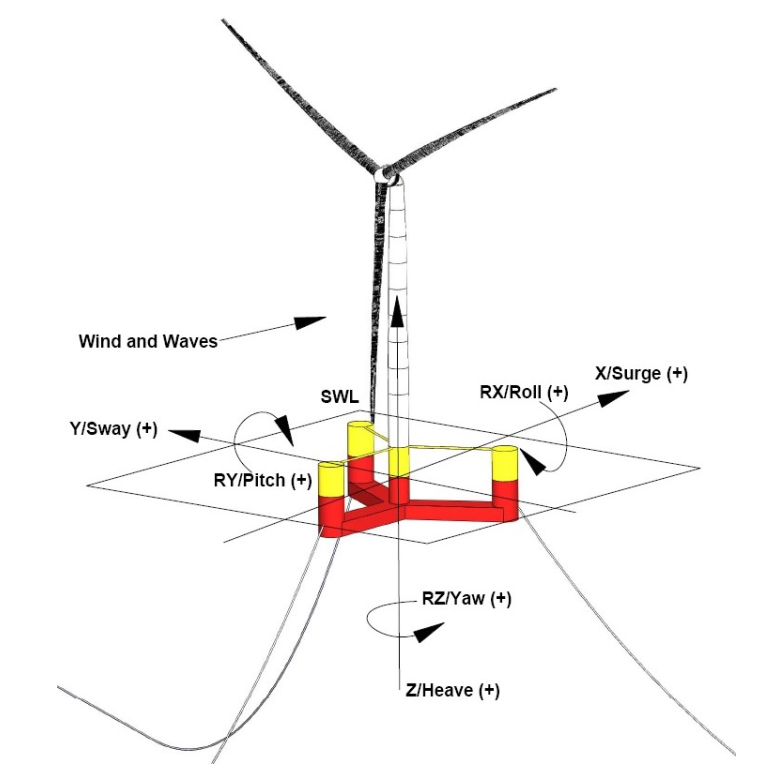
\includegraphics[width=1\linewidth]{../Graphics/FOWTcoordinates.png}
				\label{fig:fowt_coordinates}
			\end{figure}	
		\end{column}
	\end{columns}
\end{frame}

%%%%%%%%%%%%%%%%%%

\begin{frame}{Introduction}{FOWT challenges: The negative damping problem}
	
	Rotor thrust equation:
	\begin{equation} \label{eq:aero_thrust}
		F_T(\theta, \Omega, v) = \dfrac{1}{2} \rho A_d v^2 C_T(\theta, \Omega, v)
	\end{equation}
	
	\begin{columns}
		\begin{column}{.6\linewidth}
			Rotor thrust vs. wind speed with active controller:
			\begin{figure}[ht]
				\centering
				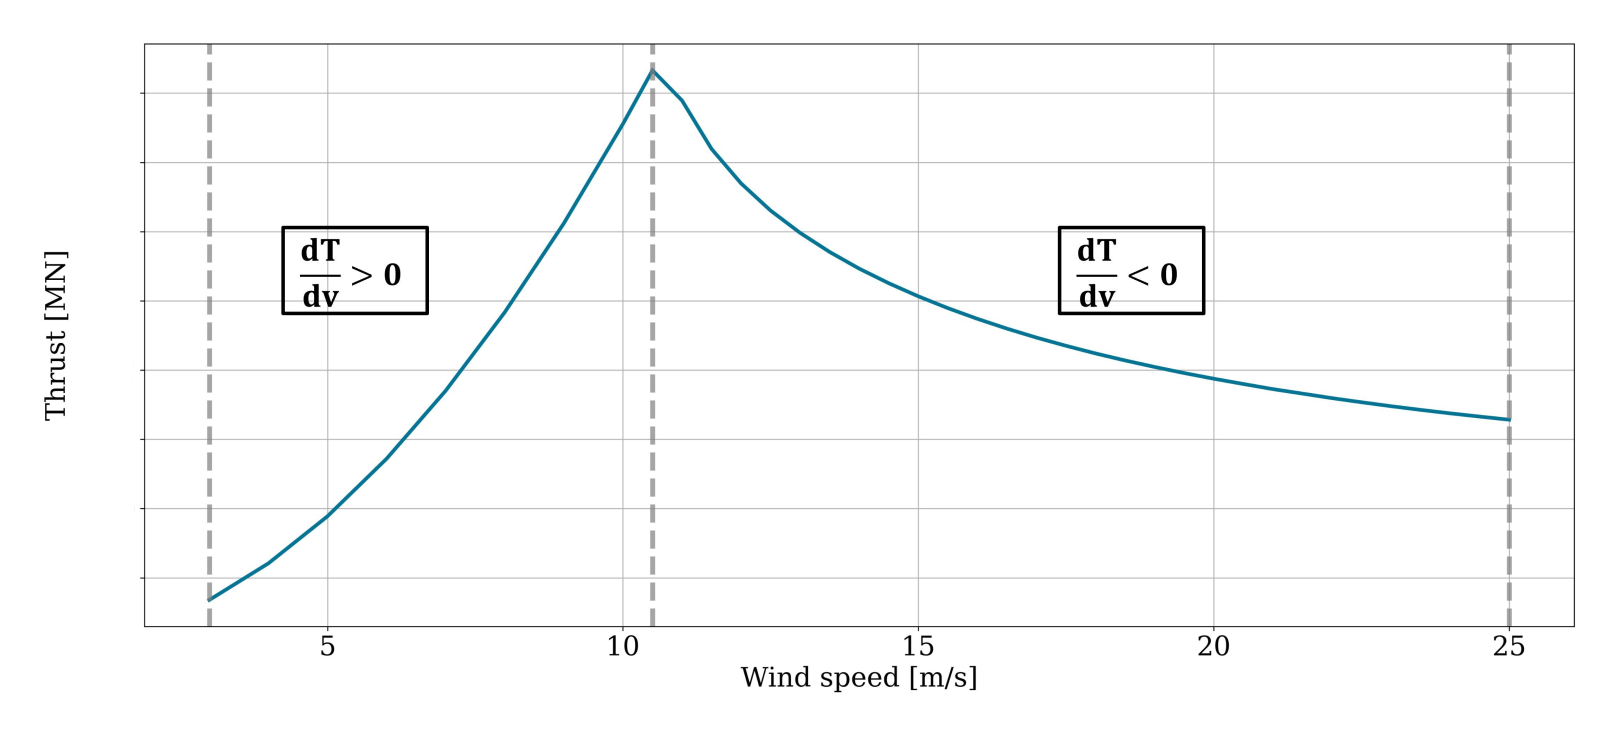
\includegraphics[width=1\linewidth]{../Graphics/ThrustWindpeedCurve.PNG}
				\label{fig:thrust_vs_windspeed}
			\end{figure}
			
		\end{column}
		\begin{column}{.4\linewidth}
			\begin{figure}[ht]
				\centering
				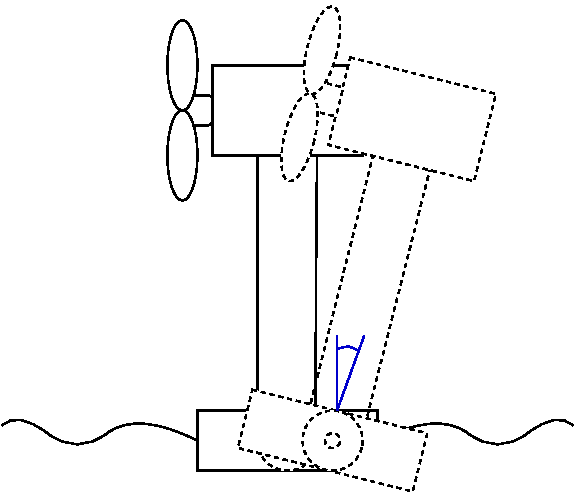
\includegraphics[width=1\linewidth]{../Graphics/ForeAftMotionModel_onlyTurbine.pdf}
				\label{fig:turbine_foreaft}
			\end{figure}
			\begin{equation*}\label{eq:vrot}
				v_{rot} = v_0 - v_y
			\end{equation*}
		\end{column}
	\end{columns}
	
\end{frame}

%%%%%%%%%%%%%%%%%%

\begin{frame}{Introduction}{The negative damping problem}
	Full-load controller and fore-aft damper have contradicting goals
	
	\smallskip
	In most FLC operating range: $ \dfrac{\partial T_r}{\partial \theta} < 0 $ but also $ \dfrac{\partial F_T}{\partial \theta} < 0 $ 
	
	\smallskip
	An example:
	\begin{enumerate}
		\item The turbine is moving forward: $ v_y < 0 $
		\item Thus $ \dfrac{\partial \Omega}{\partial v_{rot}} > 0 $ and consequently $ \Omega > \Omega_{ref} $
		\item FLC: $ \dot \theta_{ref} > 0 \rightarrow \dot \Omega < 0 $ and FATD: $ \dot \theta_{ref} < 0 \rightarrow \dot F_T > 0 $
	\end{enumerate}
	
\end{frame}

%%%%%%%%%%%%%%%%%%

%\begin{frame}{Introduction}{Wind turbine control}
%	Basic turbine controller:
%	\begin{figure}[ht]
%		\centering
%		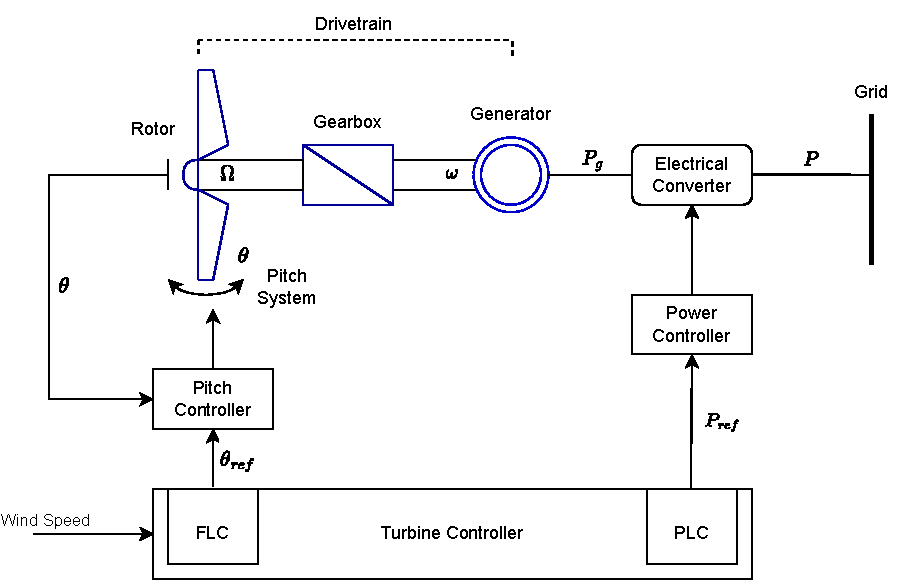
\includegraphics[width=.8\linewidth]{../Graphics/PLC_PI.pdf}
%		\label{fig:controller_overview}
%	\end{figure}
%\end{frame}

%%%%%%%%%%%%%%%%%%
%\begin{frame}{Big header}{Smaller header}
%	\textbf{Some text}
%	\begin{itemize}
%		\item Item
%	\end{itemize}
%\end{frame}
%


%%%%%%%%%%%%%%%%%%

%\begin{frame}{Big header}{Smaller header}
	%\begin{columns}
	%	\begin{column}{.49\textwidth}
	%		
	%	\end{column}
	%	
	%	\begin{column}{.49\textwidth}
	%	
	%	\end{column}
	%\end{columns}
%\end{frame}